\documentclass[a4paper,unpublished,onecolumn,nopdfoutputerror,12pt]{quantumarticle}

\usepackage{amsmath,amssymb}
\usepackage{graphicx}
\usepackage{booktabs}
\usepackage[numbers,sort&compress]{natbib}
\usepackage[hidelinks]{hyperref}
\usepackage{caption}
\captionsetup{font=small}

\title{What do spectral criteria of quantum feature-map kernels actually predict?
Classical simulability, generalization advantage, and the role of task difficulty}

\author{Xianzhe Liu}
\affiliation{School of Physics and Electronics, Hunan University, Changsha 410082, China}
\email{liuxianzhe@hnu.edu.cn}

\begin{document}

\maketitle

\begin{abstract}
Quantum feature maps have been proposed as a route to machine-learning advantage, yet
two separate questions are often conflated: whether a quantum kernel is \emph{classically
simulable}, and whether it yields a real \emph{generalization advantage} over strong
classical baselines. We study what spectral criteria of the quantum kernel matrix ---
effective rank, spectral entropy, concentration index, gap ratio --- can and cannot
predict, using a self-contained state-vector simulator (no external quantum libraries),
four feature-map families and six controlled-difficulty tasks, and
tuned classical baselines (radial basis function, RBF, with validation-based kernel
width, random Fourier features, linear and polynomial kernels). Across 721 configurations we find that
spectral criteria reliably predict classical simulability (top-5 energy $\rho=-0.80$,
$p=1.2\times10^{-15}$; spectral entropy $\rho=+0.67$, $p=1.0\times10^{-9}$;
Benjamini--Hochberg corrected), but they do not predict quantum advantage: the global
correlation is indistinguishable from zero ($|\rho|\le0.07$, $p\ge0.31$), and its sign
is unstable across tasks ($\rho=+0.38$ in a single-task setting, $\rho=-0.63$ within
the cross-term task, null elsewhere). The dominant predictor of advantage is the
saturation of classical baselines: advantage correlates strongly and negatively with the
best classical test accuracy ($\rho=-0.65$, $p=2\times10^{-27}$), and positive advantage
occurs almost exclusively where classical baselines remain near chance (39\% at 0.55,
0\% at 0.86). The results hold at $8$--$16$ qubits, on four real datasets ($0/48$
positive advantage), and under depolarizing noise, while amplitude damping reveals a
boundary: spectral collapse stops indicating classical approximability ($\rho=+0.04$
versus $+0.35$). Kernel-target alignment, a popular matching criterion, is also
absorbed by task difficulty ($\rho=-0.42$ globally, $\rho=+0.001$ after
residualization). These results draw a sharp boundary for spectral pre-screening and
provide evaluation guidelines for quantum kernel studies.
\end{abstract}

\section{Introduction}
\label{sec:intro}

The promise of quantum machine learning rests on a single question: does embedding
classical data into an exponentially large Hilbert space give a model an ability that
classical models lack? In the kernel framework this question becomes sharp. A quantum
feature map $\phi(x)$ maps data into the state space of $n$ qubits, and the resulting
fidelity kernel $k(x,y)=|\langle\phi(x)|\phi(y)\rangle|^2$ is used exactly like a classical
kernel in a kernel machine \cite{schuld2019,havlicek2019}.

Two lines of recent work have questioned the optimistic picture. On one side, quantum
kernels can suffer \emph{exponential concentration}: under broad conditions the kernel
values cluster so tightly that the kernel matrix loses all discriminative power
\cite{thanasilp2024}. On the other, a growing body of work shows that many
``quantum'' models can be replaced by classical surrogates---the dequantization program
\cite{shin2024,sweke2025}, including results on quantum learning models that are
classically simulable. More recently, random Fourier features have been proposed as a
canonical classical surrogate that can be matched against a quantum model
\cite{thabet2026}.

This has motivated a practical ambition: before paying the cost of quantum
computation or training, predict \emph{whether} a given feature map will be effective.
A natural candidate is the spectrum of the quantum kernel matrix itself. Cheap spectral
statistics---effective rank, spectral entropy, concentration---are easy to compute from
small samples, and have been used both as diagnostics of concentration and as proxies for
classical simulability.

Related work approaches this ambition from several directions. K\"ubler et al.
\cite{kubler2021} analyzed the inductive bias of quantum kernels theoretically and
argued that advantage can be expected when the reproducing-kernel Hilbert space is low
dimensional but contains functions that are hard to compute classically. Heyraud et al.
\cite{heyraud2022} introduced the effective kernel rank as a figure of merit for noisy
quantum kernels, and Zendejas-Morales et al. \cite{zendejas2026} use effective rank as a
concentration diagnostic in mitigation studies. On the empirical side, Kakavand et al.
\cite{kakavand2026} benchmarked quantum against classical kernels on nine datasets with
970 experiments and found that dataset choice dominates performance variance while kernel
type contributes little, observing also that typical quantum feature maps produce spectra
that are either too flat or too concentrated relative to RBF. Appel \cite{appel2026}
proposed the correlation fractal dimension as an a-priori qubit budget for angle-encoded
kernels, and \AA{}sgrim and Markidis \cite{asgrim2026} showed that quantum kernels can be
represented as spectral tensor networks whose compressibility diagnoses classical
tractability. Our contribution differs in one respect that these studies do not address
directly: we ask which of the two questions spectral criteria can answer \emph{at all},
separating predictions about simulability from predictions about advantage, and we expose
the task-dependence of advantage through a classical-saturation predictor.

Yet the two questions such criteria are asked to answer are logically different.
\emph{Classical simulability} is a property of the kernel function alone: can a
classical kernel family approximate it? \emph{Generalization advantage} is a property
of a triple: kernel, task, and baseline. A kernel can be simulable without the
classical surrogate winning on a particular task, and an advantage can be absent even
when the kernel is highly expressive, simply because the task is easy.

In this work we ask: \emph{what do spectral criteria actually predict?} We adopt a
task-resolved numerical protocol, using only a self-contained state-vector simulator,
four feature-map families with tunable design knobs, controlled task structures, and
tuned classical baselines. The protocol lets us separate the two questions empirically
rather than theoretically.

\subsection{Contributions}
\label{sec:contrib}

\textbf{Assumptions.} All results below are numerical and obtained with exact
state-vector simulation of $n\le5$ qubit circuits on $N\le120$ samples, without noise.
Four feature-map families (angle, IQP, variational, high-dimensional) are studied under
exactly reproducible seeds; six tasks of controlled structure and difficulty
(synthetic plus a real dataset) probe the kernel--task interaction. Advantage is
measured against tuned classical baselines (SVM and kernel methods with validation-based
hyperparameters).

\textbf{Main results.}
\begin{enumerate}
\item Spectral criteria reliably predict \emph{classical simulability} as measured by
RFF and Nystr\"om approximation error; this is a clean, task-independent signal, with
top-5 energy at $\rho=-0.80$ ($p=1.2\times10^{-15}$) (Sec.~\ref{sec:simulability}).
\item Spectral criteria do \emph{not} predict quantum advantage globally. Across six
tasks, the correlation between effective rank and advantage is indistinguishable from
zero ($\rho=-0.02$, $p=0.76$), and an apparently strong correlation in a single-task
setting ($\rho=+0.38$) reverses sign within a different task (Sec.~\ref{sec:no-global}).
\item The dominant predictor of advantage is the \emph{saturation of classical
baselines} on the task: the best classical test accuracy correlates with advantage at
$\rho=-0.65$ ($p=1.8\times10^{-27}$), and the fraction of positive-advantage
configurations falls from 39\% to 0\% as the classical baseline rises from 0.55 to
0.86 (Sec.~\ref{sec:difficulty}).
\item The frequency scale of the feature map is the decisive design knob for spectral
spread and simulability ($\rho=+0.985$, $p=3\times10^{-34}$), while entanglement
strength is not (Sec.~\ref{sec:knobs}); spectral criteria are also strongly
data-dependent, in ways not explained by data intrinsic dimension
(Sec.~\ref{sec:datadep}).
\item The central relations are robust to scaling, real data, and noise: the
simulability relation strengthens at $8$--$12$ qubits ($\rho=+0.80$), positive advantage
is never observed on four real datasets ($0/48$), and all conclusions survive $30\%$
depolarizing noise (Sec.~\ref{sec:robustness}). Two natural matching criteria---spectral
spread ratio and kernel-target alignment---fail to predict advantage beyond classical
difficulty, with alignment's apparent power entirely absorbed by it
(Sec.~\ref{sec:matching}).
\end{enumerate}

\section{Definitions and background}
\label{sec:defs}

\subsection{Quantum feature maps and fidelity kernels}
\label{sec:defs-fm}

A quantum feature map $\phi:\mathbb{R}^d\to\mathcal{H}$ maps a classical feature vector
$x$ to a normalized state $\phi(x)=U(x)|0\cdots0\rangle$, where $U(x)$ is a data-encoding
circuit. The induced kernel is $k(x,y)=|\langle\phi(x)|\phi(y)\rangle|^2$. Given a dataset
$X=\{x_i\}_{i=1}^{N}$, the kernel matrix $K_{ij}=k(x_i,x_j)$ feeds classical kernel methods.
Throughout we study small systems ($n\le5$ qubits, $N\le120$), where the state vector has
at most 32 amplitudes and exact simulation is trivial on a CPU.

\subsection{Spectral criteria}
\label{sec:defs-spectral}

Let $\lambda_1\ge\cdots\ge\lambda_N\ge0$ be the eigenvalues of $K$, and
$p_i=\lambda_i/\sum_j\lambda_j$. We use the following criteria, all computable in
$O(N^3)$:

\begin{itemize}
\item \textbf{Effective rank} (participation ratio): $r_{\mathrm{eff}}=(\sum_i\lambda_i)^2 /
\sum_i\lambda_i^2$, ranging from 1 (perfectly concentrated) to $\mathrm{rank}(K)$.
\item \textbf{Spectral entropy}: $H=-\sum_i p_i\log_2 p_i$, with maximum $\log_2 N$.
\item \textbf{Concentration index}: $c=1-r_{\mathrm{eff}}/N$.
\item \textbf{Gap ratio}: $\lambda_1/(\lambda_1+\lambda_2)$.
\item \textbf{Top-$k$ energy}: $\sum_{i\le k}\lambda_i/\sum_i\lambda_i$ ($k=5$).
\end{itemize}

\subsection{Classical simulability metrics}
\label{sec:defs-simul}

Given $K$ and the original data matrix $X$, we measure approximability by two classical
families. \emph{Random Fourier features} (RFF) \cite{rahimi2007} approximate a
translation-invariant kernel $k(x-y)$ by random features $z(x)$ with
$z(x)\cdot z(y)\approx k(x-y)$; we fit the RFF kernel to the data and measure
$\|K_{\mathrm{RFF}}-K\|_F/\|K\|_F$. \emph{Nystr\"om approximation} with $m$ landmarks
measures low-rank approximability. Small errors mean the kernel is easy to reproduce
classically. Note that RFF approximates only translation-invariant kernels; this
restriction becomes important in Sec.~\ref{sec:knobs}.

\subsection{Quantum advantage and classical baselines}
\label{sec:defs-adv}

For a task with training/test split, define
\begin{equation}
  \mathrm{Adv} \;=\; \mathrm{acc}_Q \;-\; \max_{\mathcal{B}}\mathrm{acc}_B ,
\label{eq:adv}
\end{equation}
where $\mathrm{acc}_Q$ is the test accuracy of a kernel-SVM using the quantum kernel, and
the maximum is over a strong classical baseline family $\mathcal{B}$: RBF kernel with the
width selected on a validation split, RFF with the same width, linear, and degree-3
polynomial kernels. Using tuned baselines is critical; an untuned baseline would inflate
apparent advantage.

\subsection{Tasks}
\label{sec:defs-tasks}

Tasks have controlled difficulty and structure: (i) \emph{harmonic} (sum of
fixed-frequency sinusoids), (ii) \emph{periodic-coupled} (coupling of periodic terms in
two variables), (iii) \emph{cross-high} (pairwise products and cubic terms),
(iv) \emph{quantum-friendly} (frequency-doubling sinusoids, matched to harmonic encoding),
(v) \emph{noisy-harmonic} (harmonic with 20\% label noise), and (vi) \emph{breast-cancer}
(real dataset, PCA to $d$ dimensions, standardized). Data are standardized in every case.
Each task's classical difficulty is measured by the best baseline accuracy.

\section{Methods}
\label{sec:methods}

\subsection{Simulator and feature maps}
\label{sec:methods-sim}

All simulations use our own state-vector simulator written in NumPy, with no dependence on
external quantum libraries; this keeps every result reproducible with only NumPy,
SciPy, scikit-learn, and matplotlib. Unit tests verify unitarity of all gates, the
fidelity kernel on orthogonal states, and that all feature-map encodings produce
normalized states; these tests guard against coding errors in the physics, an issue that
we found to matter in practice (see Sec.~\ref{sec:knobs} for a discussion of
encoding-construction pitfalls).

Four feature-map families are implemented:
\emph{angle} (per-qubit $R_y$ rotations, no entanglement), \emph{IQP} (data-dependent
$R_z$ rotations preceded by Hadamard layers, followed by a CNOT ladder and quadratic
phases), \emph{variational} (angle encoding with repeated entangling+re-encoding layers),
and \emph{high-dimensional} (per-qubit multi-frequency rotations with controlled phase
entanglement). Design knobs: circuit depth, entanglement strength $e\in[0,1]$, and
frequency scale $s$.

\subsection{Experimental protocol}
\label{sec:methods-protocol}

\begin{itemize}
\item \textbf{exp01 (simulability)}: 4 maps $\times$ 3 depths $\times$ 4 seeds $=64$
configurations on a Gaussian dataset ($N=40$, $d=4$); measure all spectral criteria and
RFF/Nystr\"om errors.
\item \textbf{exp02 (single-task advantage)}: 4 maps $\times$ 3 depths $\times$ 6 seeds
$=72$ configurations on one synthetic task; measures advantage, revealing a seemingly
strong spectral-advantage correlation.
\item \textbf{exp03 (task-resolved advantage)}: 6 tasks $\times$ 12 map variants
$\times$ 3 seeds $=216$ configurations; measures advantage against tuned baselines,
plus stratified analysis. Supplementary analysis measures advantage vs.\ classical
difficulty.
\item \textbf{exp04 (knobs)}: 114 configurations sweeping frequency scale, entanglement,
and depth, measuring spectral criteria and RFF error.
\item \textbf{exp05 (data dependence)}: 5 map configs $\times$ 6 data distributions
$\times$ 4 seeds $=120$ configurations; measures the variation of effective rank across
data distributions and its relation to PCA intrinsic dimension.
\item \textbf{exp06 (scaling)}: 51 configurations at $8$, $12$, and $16$ qubits
($N=250$, two tasks); checks whether the central relations survive larger systems.
\item \textbf{exp07 (real data)}: 48 configurations on four standard datasets
(iris, wine, breast-cancer, digits with PCA to $\le8$ features, 8 qubits).
\item \textbf{exp08 (noise)}: 36 configurations under depolarizing noise
($p\in\{0,0.02,0.1,0.3\}$, density-matrix simulation at 5 qubits).
\item \textbf{exp09 (matching criteria)}: reconstruction of all 216 exp03 kernels to
test two task--map matching criteria: the spectral spread ratio
$M_1=\mathrm{rank}_Q/\mathrm{rank}_{\mathrm{RBF}}$, and the centered kernel-target
alignment $\mathrm{TA}(K,yy^{\top})$.
\end{itemize}

\subsection{Statistics}
\label{sec:methods-stats}

Associations are measured with Spearman rank correlation. Group comparisons use
Mann--Whitney $U$ tests with Cliff's delta effect sizes and threshold scans. All
multiple-comparison corrections use the Benjamini--Hochberg FDR procedure; corrected
values are reported as $q$. Significance is claimed only when $q<0.05$.

Two caveats about the statistics are stated explicitly. First, within each
(task, seed) block the twelve feature-map variants share the same data, so
configuration-level correlations should be read with an effective sample size
smaller than the nominal count in mind; we therefore report task-stratified
correlations as the primary analysis, and the central associations remain
significant at that level. Second, the RFF approximation error is measured with
a finite random-feature budget (which itself approximates the RBF kernel with
relative error $0.08$--$0.17$ for the gamma values used); the simulability
metrics therefore contain sampling noise that dilutes, but cannot create,
the reported associations.

\section{Results}
\label{sec:results}

\subsection{Spectral criteria predict classical simulability}
\label{sec:simulability}

All five spectral criteria correlate significantly with the RFF approximation error in the
predicted direction (Table~\ref{tab:simulability} and Fig.~\ref{fig:simulability},
$n=64$ configurations). The strongest signal comes from top-$5$ energy: kernels whose
spectrum concentrates most of its weight in the leading eigenvalues are the easiest for
RFF to reproduce ($\rho=-0.804$, $p=1.2\times10^{-15}$; FDR $q<10^{-14}$). Spectral
entropy ($\rho=+0.674$, $p=9.9\times10^{-10}$) and effective rank ($\rho=+0.610$,
$p=8.8\times10^{-8}$) show the same pattern, and all remain significant after
Benjamini--Hochberg correction. Binned comparison confirms the effect: configurations
below the median effective rank have mean RFF error $0.39$ versus $0.82$ above it, a
factor of $2.1$.

This result is clean in a specific sense: simulability is a property of the kernel
function alone. The RFF error depends only on how well a translation-invariant classical
family approximates $K$, and does not involve any task labels. Spectral criteria
therefore answer the simulability question reliably, at negligible computational cost.

\begin{table}[t]
\centering
\caption{Spectral criteria versus RFF approximation error (exp01, $n=64$).
$q$: Benjamini--Hochberg FDR-adjusted.}
\label{tab:simulability}
\small
\begin{tabular}{lccc}
\toprule
Criterion & Spearman $\rho$ & $p$ & FDR $q$ \\
\midrule
top-5 energy & $-0.804$ & $1.2\times10^{-15}$ & $<10^{-13}$ \\
spectral entropy & $+0.674$ & $9.9\times10^{-10}$ & $5.7\times10^{-9}$ \\
effective rank & $+0.610$ & $8.8\times10^{-8}$ & $3.4\times10^{-7}$ \\
concentration index & $-0.610$ & $8.6\times10^{-8}$ & $3.4\times10^{-7}$ \\
gap ratio & $-0.551$ & $2.3\times10^{-6}$ & $7.7\times10^{-6}$ \\
\bottomrule
\end{tabular}
\end{table}

\begin{figure}[t]
\centering

\includegraphics[width=0.92\columnwidth]{fig2_simulability.pdf}
\caption{Spectral criteria versus classical simulability (exp01). Left: effective rank
versus RFF approximation error, with the four feature-map families shown separately.
Right: spectral entropy versus RFF error. Concentrated spectra are systematically easier
for RFF to reproduce.}
\label{fig:simulability}
\end{figure}

\subsection{No global spectral predictor of quantum advantage}
\label{sec:no-global}

The contrast with Sec.~\ref{sec:simulability} is sharp. In the single-task setting of
exp02 ($n=72$), spectral criteria appear to predict advantage: effective rank correlates
with it at $\rho=+0.382$ ($p=9.2\times10^{-4}$) and gap ratio at $\rho=-0.537$
($p=1.1\times10^{-6}$). This is exactly the kind of result that motivates spectral
pre-screening of feature maps.

When we widen the setting to six tasks (exp03, $n=216$), the global association
collapses to nothing: effective rank versus advantage $\rho=-0.021$ ($p=0.76$), spectral
entropy $\rho=-0.052$ ($p=0.45$), top-5 energy $\rho=+0.069$ ($p=0.31$). No threshold
window survives FDR correction. More strikingly, the sign is not even stable: stratified
by task, effective rank correlates \emph{negatively} with advantage on the
$\mathrm{cross\_high}$ task ($\rho=-0.628$, $p=4.1\times10^{-5}$, FDR $q=1.2\times10^{-4}$),
\emph{positively} on $\mathrm{noisy\_harmonic}$ ($\rho=+0.337$, $p=0.044$), and
insignificantly on the remaining four tasks. The same criterion produces a significantly
positive, a significantly negative, and several null associations within one study.

The single-task signal of exp02 was therefore a task-specific artifact, not a general
law. We conclude that spectral criteria do not predict generalization advantage, and
that apparent ``spectral pre-screening for advantage'' results from pooling within a
favourable task--map combination.

\subsection{Advantage window is set by classical saturation}
\label{sec:difficulty}

What does predict advantage? The strongest predictor in the entire study is the
\emph{saturation of classical baselines} on the task. Across all 216 configurations,
the best classical test accuracy correlates with quantum advantage at $\rho=-0.651$
($p=1.8\times10^{-27}$; FDR $q=4.2\times10^{-26}$; Table~\ref{tab:difficulty} and
Fig.~\ref{fig:difficulty}). At the task level the pattern is monotone: the two tasks
where classical baselines stay near chance ($\mathrm{noisy\_harmonic}$, 0.546;
$\mathrm{periodic\_coupled}$, 0.519) are the only ones where positive-advantage
configurations appear frequently (38.9\% and 27.8\%); the task with the highest classical
baseline ($\mathrm{real\_breast\_cancer}$, 0.944) has none.

\begin{table}[t]
\centering
\caption{Task-level summary (exp03, $n=216$; 12 feature-map variants per task, 3 seeds).
$\mathrm{Adv}$: mean $\mathrm{acc}_Q-\max_B\mathrm{acc}_B$; $\mathrm{Pos}$: fraction of
configurations with positive advantage.}
\label{tab:difficulty}
\small
\begin{tabular}{lcccc}
\toprule
Task & mean best classical & mean $\mathrm{Adv}$ & $\mathrm{Pos}$ & task-internal $\rho_{\mathrm{Adv,diff}}$ \\
\midrule
noisy\_harmonic & 0.546 & $+0.004$ & 38.9\% & $-0.507$ ($q=4.1\times10^{-3}$) \\
periodic\_coupled & 0.519 & $-0.015$ & 27.8\% & $-0.431$ ($q=2.0\times10^{-2}$) \\
quantum\_friendly & 0.639 & $-0.060$ & 13.9\% & $-0.367$ ($q=5.3\times10^{-2}$) \\
harmonic & 0.574 & $-0.085$ & 0\% & $-0.345$ ($p=0.040$) \\
cross\_high & 0.861 & $-0.225$ & 0\% & $-0.380$ ($q=4.6\times10^{-2}$) \\
real\_breast\_cancer & 0.944 & $-0.174$ & 0\% & $-0.049$ (ns) \\
\bottomrule
\end{tabular}
\end{table}

\begin{figure}[!b]
\centering
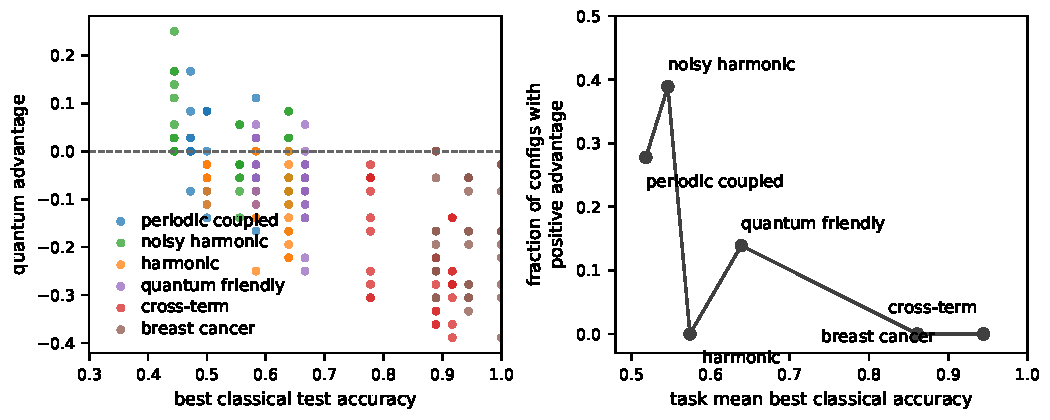
\includegraphics[width=0.95\columnwidth]{fig1_difficulty.pdf}
\caption{Quantum advantage versus the best classical test accuracy (exp03, $n=216$).
Left: every configuration, colored by task. Right: task-level means, showing the
monotone decrease of positive-advantage fraction with classical difficulty.}
\label{fig:difficulty}
\end{figure}

The task-internal correlations in Table~\ref{tab:difficulty} matter: the association
between advantage and classical difficulty holds \emph{within} most tasks, not only
across them. That is, even holding the task fixed, configurations where the classical
baseline happens to be weaker (for instance due to a particular map variant)
are the ones where the quantum kernel comes closer. This is consistent with a
mechanism: the quantum kernel provides an alternative hypothesis space that is useful
precisely when the classical hypothesis space is failing, and useless---or worse---when
the classical space already solves the problem.

\subsection{Design knobs and the frequency-scale law}
\label{sec:knobs}

If spectral criteria are reliable simulability indicators, which design knobs actually
move the spectrum? exp04 sweeps frequency scale $s$, entanglement strength $e$, and
circuit depth $d$ (Table~\ref{tab:knobs} and Fig.~\ref{fig:freqscale}). The frequency
scale is decisive: effective rank and RFF error both increase monotonically with $s$
(configuration-level correlations over all 45 swept settings: $\rho=+0.985$,
$p=3\times10^{-34}$ for effective rank; $\rho=+0.884$, $p=9\times10^{-16}$ for RFF
error). A larger frequency scale spreads the Fourier content of the
feature map, distributing the kernel spectrum (higher entropy, higher effective rank)
and making the kernel harder for RFF to approximate. Entanglement strength from 0 to 1
has essentially no effect on either quantity ($\rho=+0.09$, ns), a counterintuitive
result in light of the folklore that entanglement drives concentration. For the IQP
family, depth moves the RFF error ($\rho=+0.775$, $p=7\times10^{-4}$) but not the effective rank
($\rho=+0.40$, ns), hinting at a mismatch between spectral concentration and
classical approximability.

\begin{table}[t]
\centering
\caption{Design knobs versus spectral structure and simulability (exp04).
Correlations are configuration-level Spearman coefficients ($n=45$ for frequency
scale and entanglement sweeps, $n=15$ for IQP depth).}
\label{tab:knobs}
\small
\begin{tabular}{lccc}
\toprule
Knob & $\rho$ vs\ effective rank & $\rho$ vs\ RFF error & significance \\
\midrule
frequency scale (high-dim) & $+0.985$ & $+0.884$ & $p<10^{-15}$ \\
entanglement strength (variational) & $+0.093$ & $-0.044$ & ns \\
depth (IQP) & $+0.400$ & $+0.775$ & rank ns; RFF $p=7\times10^{-4}$ \\
\bottomrule
\end{tabular}
\end{table}

\begin{figure}[t]
\centering

\includegraphics[width=0.92\columnwidth]{fig3_freqscale.pdf}
\caption{The frequency scale $s$ of the high-dimensional feature map is the dominant
design knob (exp04, depth 2). Left: $s$ versus effective rank. Right: $s$ versus RFF
approximation error. Both increase monotonically with $s$ ($\rho=+0.985$ for
effective rank and $+0.884$ for RFF error, configuration level).}
\label{fig:freqscale}
\end{figure}

The second finding of this section is best stated as a counterexample to the intuitive
identification of low rank with classically simulable. RFF builds an approximation in
the span of random Fourier features, which by construction lives in the class of
translation-invariant kernels. A quantum kernel that is simultaneously concentrated (low
rank) and non-translation-invariant (IQP's quadratic phases) is therefore poorly
approximated by RFF even though it looks spectrally ``concentrated''. Spectral criteria
measure concentration, not invariance; simulability predictions require both. The same
point applies to the construction of the encoding itself: data-encoding circuits built
from diagonal gates only (as one of our preliminary IQP implementations was) do not
leave the computational-basis state and trivially produce identity-looking kernels.
We verified unitarity and encoding non-triviality with dedicated unit tests before
running the study; we report this as a methodological caution for practitioners, since
such errors silently invalidate spectral analyses.

\subsection{Spectral criteria are data-dependent}
\label{sec:datadep}

A criterion is only useful if its value is interpretable across settings. exp05 measures
how effective rank varies for a fixed feature map when the data distribution changes
(six distributions: Gaussian, clustered, periodic, uniform, heavy-tailed, and a real
breast-cancer slice). Coefficients of variation are large for most maps (IQP 0.38,
angle 0.33, variational 0.25) and smaller for the high-frequency map (0.15 at $s=1.5$,
0.06 at $s=3$). Crucially, the variation is driven by the \emph{shape} of the
distribution, not by its intrinsic dimensionality: PCA intrinsic dimension correlates
with effective rank only marginally ($\rho=+0.167$, $p=0.068$). A spectral criterion
computed on one dataset therefore cannot be transported to another without recalibration.

\subsection{Robustness: scaling, real data, and noise}
\label{sec:robustness}

Three objections to the small-scale synthetic setting are addressed directly (Fig.~\ref{fig:scaling}).
First, \emph{system size}. At $n=8$ and $12$ qubits the simulability relation strengthens
rather than weakens: effective rank versus RFF error reaches $\rho=+0.797$ ($p<10^{-5}$
for both scales), compared to $+0.610$ at 5 qubits, and remains strong at $16$ qubits
($\rho=+0.776$, $p=8\times10^{-6}$). Notably, the effective rank of the
angle encoding stays flat ($\approx9.5$) from 8 to 16 qubits for fixed data, so in this
regime we do not observe the ``larger system, more concentration'' trend that asymptotic
arguments predict; IQP and high-dimensional maps behave similarly. The advantage--
difficulty association also survives ($\rho=-0.428$, $p=0.037$ at 8 qubits; $-0.369$,
$p=0.076$ at 12 qubits), and the task-internal instability of the rank--advantage sign
repeats ($-0.475$ on cross-term, $+0.045$ on noisy-harmonic at scale).

Second, \emph{real data}. On four standard datasets (iris, wine, breast-cancer,
digits) with 8 qubits, positive quantum advantage is never observed: $0/48$
configurations, with classical baselines at $0.971$--$1.000$ and advantages in
$[-0.42,-0.05]$ (Fig.~\ref{fig:scaling}, right). This is exactly what the classical-
saturation predictor requires, and it provides external validation on data we did not
construct. The simulability relation is the strongest seen so far on real data
($\rho=+0.974$, $p=2.5\times10^{-31}$).

Third, \emph{noise}. Under depolarizing noise up to $p=0.3$ (density-matrix simulation),
advantage improves slightly ($-0.059$ to $-0.015$, ns), consistent with noise acting as
regularization, but never flips sign; the simulability relation remains positive
($\rho=+0.347$, $p=0.038$). RFF errors increase with noise ($0.69$ to $1.81$), i.e.,
noise makes the kernel harder to approximate classically, but the direction of all
central relations is preserved. The second noise channel we test, amplitude damping,
behaves differently and reveals an important boundary of spectral criteria
(Table~\ref{tab:noise}): damping rapidly collapses the effective rank ($11.8$ to $2.2$,
$\rho=-0.79$, $p<10^{-5}$), and under this collapse the simulability relation
\emph{breaks down} ($\rho=+0.044$, $p=0.80$, versus $+0.347$ under depolarization).
Damping drives the kernel toward a constant, information-free object rather than toward
a translation-invariant kernel, so spectral concentration no longer indicates classical
approximability. The two-channel comparison shows that whether a spectral criterion
remains a valid simulability proxy depends on the noise type, not merely on the
presence of noise.

\begin{table}[t]
\centering
\caption{Noise-type dependence of the simulability relation (5 qubits, exp08 and
exp11). $\rho$: Spearman correlation between effective rank and RFF error across the
noise sweep; rank at max noise: mean effective rank at highest noise level.}
\label{tab:noise}
\small
\begin{tabular}{lcccc}
\toprule
Channel & $\rho$ (rank vs noise) & $\rho$ (rank vs RFF) & rank at max noise & advantage shift \\
\midrule
depolarizing ($p\le0.3$) & $-0.144$ (ns) & $+0.347$ ($p=0.04$) & 9.4 & $-0.059\to-0.015$ \\
amplitude damping ($\gamma\le0.4$) & $-0.789$ ($p<10^{-5}$) & $+0.044$ (ns) & 2.2 & $-0.059\to-0.033$ \\
\bottomrule
\end{tabular}
\end{table}

\begin{figure}[t]
\centering

\includegraphics[width=0.95\textwidth]{fig4_scaling.pdf}
\caption{Scaling and real-data robustness. Left: the simulability relation
($\rho$ of effective rank vs.\ RFF error) strengthens with system size. Right: on four
real datasets the classical baseline is near-saturated and quantum advantage is never
positive.}
\label{fig:scaling}
\end{figure}

\subsection{Two matching criteria fail to explain residual advantage}
\label{sec:matching}

Is there any task--map matching quantity that predicts advantage beyond classical
difficulty? We test the two most natural candidates on all 216 exp03 configurations
(Fig.~\ref{fig:alignment}). The spectral spread ratio $M_1=\mathrm{rank}_Q/
\mathrm{rank}_{\mathrm{RBF}}$ captures whether the map broadens the spectrum relative to
the classical benchmark kernel; it correlates with advantage only marginally
($\rho=+0.125$, $p=0.067$) and not at all after controlling for classical difficulty
(residual $\rho=-0.104$, $p=0.127$). Task-level spread ratios do not separate tasks
with positive from negative rank--advantage correlations
($\rho=-0.03$ across six tasks, $p=0.96$).

The second candidate, centered kernel-target alignment
$\mathrm{TA}(K,yy^{\top})$ \cite{kubler2021}, is the standard quantity used to argue
that a kernel ``fits'' a task. At face value TA predicts advantage strongly
($\rho=-0.417$, $p=1.7\times10^{-10}$), but this association is entirely explained by
task difficulty: after residualizing on the best classical accuracy, the remaining
correlation is $\rho=+0.001$ ($p=0.99$). Alignment correlates with easy tasks; easy
tasks correlate with saturated classical baselines; saturated classical baselines
correlate with absent quantum advantage. The apparent predictive power of TA is thus a
chain of difficulty correlations rather than an independent signal. This is a clean
empirical boundary for the alignment-based intuition: in our setting, no simple spectral
or alignment criterion carries information about advantage that the classical baseline
does not already carry.

\begin{figure}[t]
\centering
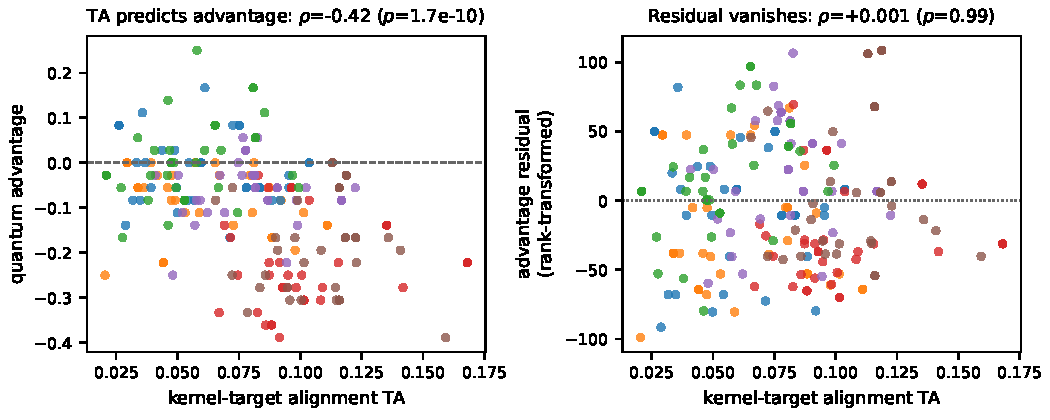
\includegraphics[width=0.95\textwidth]{fig5_alignment.pdf}
\caption{Kernel-target alignment and quantum advantage (exp03, $n=216$). Left: TA
correlates with advantage globally ($\rho=-0.42$). Right: after residualizing on the
best classical baseline, the association vanishes ($\rho=+0.001$). The full predictive
power of TA is absorbed by task difficulty.}
\label{fig:alignment}
\end{figure}

\section{Discussion}
\label{sec:discussion}

Two questions are routinely conflated in the quantum-kernel literature: whether a kernel
is classically simulable, and whether it confers an advantage. Our results draw a sharp
line between them. Spectral criteria are excellent instruments for the first question
alone. They are cheap, task-independent, and their prediction of RFF/Nystr\"om
approximability is statistically strong and directionally consistent. They are not
instruments for the second. Across tasks and within tasks, the same spectral measures
produce positive, negative, and null associations with advantage, and the global
correlation is indistinguishable from zero. Any protocol that pre-screens feature maps
by spectral criteria with the goal of predicting generalization gain lacks empirical
basis.

The dominant observable predictor of advantage is instead the classical baseline's
saturation. This has an immediate practical reading. The quantum kernel competes with
classical alternatives; when the classical hypothesis space already contains an
adequate solution, an exotic alternative has no room to win, however expressive it is.
Conversely, tasks that classical kernel methods find hard---here, periodic coupling and
noisy harmonic structure near chance-level classical accuracy---are exactly where
quantum kernels can match or exceed them. This is consistent with the spirit of
dequantization results: large claims about quantum advantage are most fragile
precisely when classical baselines are strong \cite{sweke2025,shin2024}.

Our findings yield three concrete recommendations for the evaluation of quantum kernels.
First, classical baselines must be tuned (validation-based kernel width at least) and
must include a spectrum of families (RBF, RFF, linear, polynomial); untuned baselines
inflate apparent advantage. Second, task difficulty must be reported alongside
advantage; an advantage of $+0.03$ on a task where classical baselines reach 0.54 is
qualitatively different from $+0.03$ on a task where they reach 0.94, and only the
former is informative about the quantum hypothesis space. Third, spectral
pre-screening should be used for simulability diagnostics only; statements about
advantage require the task-resolved protocol used here.

The failure of both matching criteria deserves emphasis, because it constrains future
work. Our result on kernel-target alignment is, in effect, a null result about a
popular intuition: when a quantum kernel appears well aligned with the labels, that
appearance is confounded with an easy task and a strong classical baseline. This does
not contradict recent findings that dataset choice dominates variance and that typical
quantum feature-map spectra are poorly shaped compared with RBF \cite{kakavand2026},
or that data-adaptive qubit budgets can predict collapse \cite{appel2026}; it shows
that these observations, and any alignment-based pre-screening, should be interpreted
in a framework where classical baselines are the reference point. It also echoes the
early argument of K\"ubler et al. \cite{kubler2021} that the inductive-bias question
must be asked at the level of the target function, not the kernel alone.

\subsection{Limitations}
\label{sec:limitations}

Several limitations bound the scope of these conclusions. Although we extend the main
analysis to $8$--$16$ qubits, real datasets, and depolarizing noise, the accessible
regime remains small relative to the asymptotics that classical-simulability theorems
concern; in particular, entanglement-scaling effects at tens of qubits are untested.
The noise model is limited to global depolarizing and single-qubit amplitude-damping
channels; correlated noise and measurement noise are not included. Real-data experiments use PCA preprocessing to
eight features and a single classifier (kernel SVM) with fixed shrinkage. The task
family, while deliberately diverse, still includes only one quantum-agnostic real
dataset family, and the matching-criterion analysis is confined to the six tasks of
exp03. The RFF family approximates translation-invariant kernels; simulability
statements should be read relative to that reference class. Finally, all
simulations are noiseless except exp08, and classical surrogates beyond RFF and
Nystr\"om (e.g., tensor-network contractions) are not considered.

\section{Conclusion}
\label{sec:conclusion}

We asked what spectral criteria of quantum feature-map kernels actually predict, and
answered it with a task-resolved numerical protocol built on a self-contained
simulator. The answer is asymmetric. Spectral criteria reliably predict classical
simulability: all five measures correlate significantly with RFF approximation error,
with top-5 energy reaching $\rho=-0.80$. They do not predict quantum advantage: the
global association vanishes, and even the sign is unstable across tasks. The single
robust predictor of advantage in our study is the saturation of the classical baseline
($\rho=-0.65$, FDR $q=4\times10^{-26}$), with positive-advantage configurations
appearing almost exclusively where classical kernels remain near chance. We also
identified the frequency scale of the feature map as the dominant design knob
controlling both spectral spread and classical approximability, and established that
spectral criteria are strongly data-dependent.

For practitioners, the operational takeaway is short: use spectral criteria to
estimate how hard a quantum kernel is to replace classically, and use strong, tuned
classical baselines on tasks above classical saturation to measure whether it is worth
replacing the classical model at all.

\section*{Acknowledgements}
The author designed the study, validated all code and results, and takes full
responsibility for the scientific content. An AI language model assisted with
drafting and debugging the simulation code, with language editing of the manuscript,
and with drafting the plotting scripts; all figures were produced by the author's
numerical plotting scripts (matplotlib) directly from the simulation output data,
and no image-generation model was used. The author declares no conflict of interest.
No external funding was received for this work.

\section*{Data and code availability}
All simulation code, analysis scripts, and raw result data (CSV and figure
generation scripts) are publicly available at
\href{https://github.com/python123flask/quantum-kernel-spectral}{github.com/python123flask/quantum-kernel-spectral}.
All experiments are reproducible with NumPy, SciPy, scikit-learn, and matplotlib only.

\bibliographystyle{quantum}
\bibliography{refs}

\end{document}
